\section{Evaluation}\label{sec:eval}

In this section, we estimate the concrete costs of our protocols. We start with the symmetric \ourprotocol\ and \ourprotocoltwo\ (\Cref{sec:symmetriceval}) and then continue with the asymmetric \sqrtmergeprotocol\ and \knmergeprotocol\ (\Cref{sec:asymmetriceval}).
We consider input lists of size $n = 2^{20}$ with $\ell = 128$ bit elements, and express the cost in terms of: (1) the number of comparisons, and (2) the number of rounds due to comparisons. For the number of rounds, we assume GMW-style comparisons, which require $\log \ell$ rounds. For the asymmetric protocols, we adjust the size of one list to $n^{\frac{1}{2}}$ and $n^{\frac{1}{3}}$, respectively.
Note that we estimated the total bandwidth cost, with secure comparisons being the primary bottleneck, responsible for more than 90\% of the total bandwidth in all our protocols except the \sqrtmergeprotocol\ protocol. Furthermore, since our protocols are described at a low level, essentially as pseudocode, we do not expect any additional significant costs that are unaccounted for in our analysis.





We benchmark our protocols against the state-of-the-art Batcher's network merge and shuffle-then-sort (see \Cref{sec:relwork}) . Recall that the shuffle-then-sort technique concatenates $\X||\Y$, shuffles them, and then uses some secure sort such as quick-sort \cite{ICISC:HKICT12,EPRINT:PRRS23}.
To sort a list of size $n = n_0+n_1$ with $\ell$-bit elements via quick-sort, we require $O(n\log n)$ secure comparisons and $O(\log n \log \ell)$ rounds. We use $1.44$ for constant (empirical constant resulting in $1.44\cdot n\log n$ comparisons), originating from the choice of pivots to partition the sub-arrays. 
In Batcher's network, we use $\frac{n}{2}\log n$ comparisons and $(1+\log n) \log \ell$ rounds.
For completeness, we also include the costs of \cite{EPRINT:BBDLO22} when evaluating our symmetric protocols, despite their large constants.
More specifically, we include \cite{EPRINT:BBDLO22}'s costs for their (1) full protocol, and also for their (2) $\Pi_{\textsf{SSM-}{\log}{\log} n}$ subprotocol (Step 1 in our high-level description of \cite{EPRINT:BBDLO22} in \Cref{sec:bbdlosecuremerge}), which also merges two arbitrary lists of length $n$, but is used only as a subprotocol of \cite{EPRINT:BBDLO22}'s full protocol.

The recent advancements in the non-comparison-based radix sort \cite{EPRINT:PRRS23}, enabled by its efficient 2-party permutation, have significantly improved its practicality. This approach requires $2\ell$ rounds, making it comparable to our method only for small $\ell$ (cf. \Cref{fig:mergeconcrete}). However, it incurs a computational cost of $n\ell\kappa^2$, which, while linear, becomes substantial given a typical security parameter of $\kappa \approx 128$. Additionally, in terms of communication, radix sort still requires $O(n\ell\log n)$, resulting in considerable overhead relative to our approach. We exclude it from further comparison.

\subsection{\ourprotocol\ and \ourprotocoltwo\ Evaluation}\label{sec:symmetriceval}

We first evaluate our symmetric protocols. We present our findings in \Cref{fig:mergeconcrete}, then interpret our results, and discuss some key aspects of our cost estimates.
%assumptions and protocol changes we make for our cost estimates. %For details of our \ourprotocol\ and \ourprotocoltwo\ costs see \Cref{sec:costdetails}. 

\renewcommand{\arraystretch}{1.2}
\begin{figure}[!h]\small
    \centering
    
    \begin{tabular}{|l|c|c|}
    \hline\textbf{Protocol} & \textbf{\# Comparisons} & \textbf{\# Rounds}\\
    \hline \hline
    \cite{EPRINT:BBDLO22}'s Full Protocol & $1.27 \cdot 10^8$ & 483\\
    \hline    \cite{EPRINT:BBDLO22}'s Subrotocol $\Pi_{\textsf{SSM-}{\log}{\log} n}$ & $1.15 \cdot 10^8$ & 179\\
    \hline
        (Shuffled) Quick-Sort & $6.34 \cdot 10^7$ & 212\\
    \hline
        Batcher's Network & $2.20 \cdot 10^7$ & 154\\
    \hline
    \hline
   \ourprotocol & $\mathbf{1.53 \cdot 10^7}$ & 155\\ 
    \hline
    \ourprotocoltwo & $5.43 \cdot 10^7$ & \textbf{118}\\
    \hline    \end{tabular}
    \caption{Comparison of our protocols \ourprotocol\ and \ourprotocoltwo\ with the state-of-the-art merge techniques. We let the input length $n=2^{20}$ and the element bitlength $\ell=128$. We express our cost in terms of number of comparisons and the number of rounds due to comparisons, which we discover is a bottleneck in our protocols.}
    \label{fig:mergeconcrete}
\end{figure}

\paragraph{\Cref{fig:mergeconcrete} Results Interpretation.} For $n=2^{20}$, \ourprotocol\ reduces the number of comparisons $\approx 1.4\times$ over Batcher's network and $\approx4.1\times$ over shuffle-then-sort. It achieves this without significantly increasing the number of rounds. To compute the comparisons, \ourprotocol\ uses $155$ rounds, while Batcher's network uses $154$ and shuffle-then-sort $212$. We note that for a larger input, \ourprotocol's improvement becomes more pronounced due to superior asymptotics. E.g., for $n=2^{30}$, \ourprotocol, with $1.69\cdot10^{10}$ comparisons, reduces the number of comparisons $\approx 2.0\times$ over Batcher's network and $\approx5.7\times$ over shuffle-then-sort.\footnote{We note that databases with $n \geq 2^{30}$ are not uncommon. For example, such large datasets are frequently found in areas like network traffic monitoring, financial transactions, and online advertising data.} At the same time, \ourprotocol\ uses 239 rounds, whereas Batcher's network uses 224 rounds and shuffle-then-sort uses 313 rounds. \ourprotocoltwo\ provides a tradeoff between bandwidth and rounds. For $n = 2^{20}$, it increases the number of required comparisons $\approx 2.5\times$ over Batcher's network while still decreasing them $\approx 1.2\times$ over shuffle-then-sort, but decreases the number of rounds over both, i.e. $\approx 1.3\times$ over Batcher's network and $\approx 1.8\times$ over shuffle-then-sort. For $n=2^{30}$, \ourprotocoltwo, with $7.45\cdot10^{10}$ comparisons, increases bandwidth $\approx2.2\times$ over Batcher's network while still decreasing it $\approx1.3\times$ over shuffle-then-sort, but decreases the number of rounds over both, namely $\approx1.5\times$ over Batcher's network and $\approx2.1\times$ over shuffle-then-sort. Hence, \ourprotocoltwo\ is suitable for high-latency networks. \cite{EPRINT:BBDLO22} stresses superior asymptotics, but is concretely less efficient even than shuffle-then-sort. With respect to \ourprotocol\ and $n=2^{20}$, it uses $\approx8.3\times$ more comparisons and $\approx3.1\times$ more rounds. \cite{EPRINT:BBDLO22}'s $\Pi_{\textsf{SSM-}{\log}{\log} n}$ subprotocol (Step 1 in \Cref{sec:bbdlosecuremerge}), which also serves as a standalone symmetric merge, uses $\approx7.5\times$ more comparisons than \ourprotocol\ and $\approx1.2\times$ more rounds. \\ %Recall from  our discussion in \Cref{sec:relworkmerging} that we significantly underestimate \cite{EPRINT:BBDLO22}'s costs. We expect the difference to be much larger. \\

\noindent We now discuss key aspects of our cost estimates. %assumptions and protocol changes we make to compute our costs. 
We start with \ourprotocol, continue with \ourprotocoltwo, and then finish with \cite{EPRINT:BBDLO22}.

\paragraph{\ourprotocol.}

We follow \ourprotocol\ as defined in \Cref{fig:ourprotocol} except we set the block size $m:=7$ instead of $\log\llength$. In the base case, we then use \cite{TCS:MI04}'s merging network that requires $21$ comparisons for inputs of size $7$ (which is slightly less than Batcher's network).\footnote{For $n=2^{30}$, we use $m = 8$ and a merging network with 25 comparisons \cite{TCS:MI04}.} Note that with this change, we execute both the recursive step and the base case once.
To sort medians in step \ref{ourprotocolrecursivestep2b}, we use Batcher's network.

\paragraph{\ourprotocoltwo.} 

We follow our algorithm almost exactly as in \Cref{fig:ourprotocoltwo}. Our only deviations are in the base case where we increase the size of the base case so that we finish recursion after exactly $2$ steps for both $n=2^{20}$ and $n=2^{30}$. We use Batcher's network \cite{AFIPS:Bat68} in the base case.

\paragraph{\cite{EPRINT:BBDLO22}.} We note that their protocol is highly optimized with respect to asymptotics. We do not see any simple way to optimize their protocol for concrete efficiency.

%\noindent We finish recursion after exactly $\log\log n$ step when we reach the base case.


\subsection{\sqrtmergeprotocol\ and \knmergeprotocol\ Evaluation}\label{sec:asymmetriceval}

Next, we evaluate our asymmetric protocols. We first evaluate \sqrtmergeprotocol, then we evaluate \knmergeprotocol.
For each protocol, we present our findings and interpret our results. %, and discuss key aspects our cost estimates.

\paragraph{\sqrtmergeprotocol.} See our results in \Cref{fig:sqrtmergeconcrete}. We present the costs for the exact same algorithm as in \Cref{fig:sqrtmergeprotocol}.

\begin{figure}[!h]\small
    \centering
    
    \begin{tabular}{|l|c|c|}
    \hline\textbf{Protocol} & \textbf{\# Comparisons} & \textbf{\# Rounds (Agg. Tree and Comparisons)}\\
    \hline \hline
        (Shuffled) Quick-Sort & $3.02\cdot10^7$ & 202\\
    \hline
        Batcher's Network & $1.05\cdot 10^7$ & 147\\    
    \hline
   \sqrtmergeprotocol & $\mathbf{2.10\cdot10^6}$ & $\mathbf{56}$\\ 
    \hline\end{tabular}
    \caption{Comparison of \sqrtmergeprotocol\ with the state-of-the-art merge techniques. We let $n=2^{20}$ and set the length of the input lists to $n^{\frac{1}{2}}$ and $n$, respectively. We express our cost in terms of number of comparisons and the number of rounds due to comparisons and aggregation trees (as comparisons are not a bottleneck for round complexity in \sqrtmergeprotocol).}
    \label{fig:sqrtmergeconcrete}
\end{figure}

\paragraph{\Cref{fig:sqrtmergeconcrete} Results Interpretation.}
While for the symmetric protocols and our \knmergeprotocol\ comparisons constitute an overwhelming cost, this is not quite true for \sqrtmergeprotocol. We estimate comparisons make up $\approx50\%$ of the total bandwidth cost. 
Hence, while we decrease the number of comparisons $\approx5\times$ over Batcher's merge, we estimate our bandwidth is $\approx2.5\times$ smaller. For the rounds, aggregation trees in combination with the comparisons are the overwhelming bottleneck. We thus combine the round cost for the comparisons and the aggregation trees to estimate the total cost. We get a $\approx2.6\times$ improvement over Batcher's merge. 

\paragraph{\knmergeprotocol.} See our results in \Cref{fig:knmergeconcrete}. We present the costs for the exact same algorithm as in \Cref{fig:knmergeprotocol}. Note that a similar performance was already achieved by \cite{EPRINT:BBDLO22}'s protocol, but did not have concrete estimates. Our \knmergeprotocol\ is highly similar to that protocol, but is modified and expressed in our notation. %\stan{please check this sentence is sensible}

\begin{figure}[!h]\small
    \centering
    
    \begin{tabular}{|l|c|c|}
    \hline\textbf{Protocol} & \textbf{\# Comparisons} & \textbf{\# Rounds}\\
    \hline \hline
        (Shuffled) Quick-Sort & $3.02\cdot10^7$ & 202\\
    \hline
        Batcher's Network & $1.05\cdot 10^7$ & 147\\    
    \hline
   \knmergeprotocol & $\mathbf{2.11\cdot10^6}$ & $\mathbf{23}$\\ 
    \hline\end{tabular}
    \caption{Comparison of \knmergeprotocol\ with the state-of-the-art merge techniques. We let $n=2^{20}$ and set the length of the input lists to $n^{\frac{1}{3}}$ and $n$. As in \Cref{fig:mergeconcrete}, we express our cost in terms of number of comparisons and the number of rounds due to comparisons.}
    \label{fig:knmergeconcrete}
\end{figure}

\paragraph{\Cref{fig:knmergeconcrete} Results Interpretation.}  \knmergeprotocol\ reduces the number of comparisons $\approx5.0\times$. This corresponds to approximately the same bandwidth reduction. For the number of rounds, we estimate that comparisons count for $\approx\frac{2}{3}$ of the total rounds. Hence, we estimate we reduce the total round complexity $\approx 4.3\times$. 

% TOTAL IN WOLFRAM ALPHA: 40 log_2 40 *  ceiling(2^20 / 20 * 2) + (2 * 2^20 / 20) log_2 (2 * 2^20 / 20) + ( 2 * 2^20 / 20) * 20 * 3
















% We assume the bitlength of the list elements is $l = 128$ and the security parameter $\kappa = 128$.
% We now show how we estimate the cost for \ourprotocol\ and \ourprotocoltwo\ for $n=2^{10}$; the estimates for the remaining $n$ can be derived similarly and are presented in \stan{table X}.

% \paragraph{\ourprotocol\ (see \Cref{fig:ourprotocol}).}

% We first evaluate the cost of \ourprotocol; then we evaluate the recursive method \ourprotocolrecursive.

% \begin{itemize}
%     \item \ourprotocol: Steps \ref{ourprotocolstep1}-\ref{ourprotocolstep3} require no interaction. Step \ref{ourprotocolstep4} is complex, and hence we evaluate separately below. Step \ref{ourprotocolstep5} invokes \extractinorderprotocol\ \cite{EPRINT:PRRS23}, which requires $3$ rounds and communicates $4\llength\kappa = 64$KB of communication. Note $4n$ is the length of the output returned from the recursive \ourprotocolrecursive\ as we reach base just after a single invocation ($\log_2 2^{10}=10 \leq 10$).
%     \item \ourprotocolrecursive: We invoke \ourprotocolrecursive\ twice. The first invocation invokes the recursive step; the second invocation invokes the base case. We now evaluate them separately:
%     \begin{itemize}
%         \item  \textbf{Base Case:}
%         When we reach base case $n=10$. Step \ref{ourprotocolrecursivestep1a} invokes \mergeallpairsprotocol, which requires $n^2 = 100$ secure comparisons. Secure comparison for $l$-bit inputs and implemented with GMW requires $l\log l$ bits of communication and $\log l$ rounds. Hence, this step costs $n^2 l \log l \approx 10.94$KB and $\log l = 7$ rounds.
%         Step \ref{ourprotocolrecursivestep1b} invokes \executemergeinvprotocol\ \cite{EPRINT:PRRS23},  which costs $2$ rounds and $2nl'$ bits of communication, where $l'$ is bitlength rounded up to $\kappa$ and $2n$ is the length of the appended \X\ and \Y. In our case, this corresponds to $\approx0.31$KB of communication. Note that this can be significantly optimized as we permute indices that are much less than $128$ bits, which would allow us to reuse parts of permutation correlations in practice (\cite{EPRINT:PRRS23}). For example, $32$-bit indices would allow us to use $128-32$ remaining bits of the correlation.
%         Thus, steps \ref{ourprotocolrecursivestep1a}-\ref{ourprotocolrecursivestep1b} cost $11.25$KB and $9$ rounds.
%         Note that the base case is evaluated in parallel for $2\lceil k \rceil = 206$ subproblems. Thus, the total base case cost is $9$ rounds and $\approx2317.5$KB.
%         \item \textbf{Recursive Step:} The recursive step \ref{ourprotocolrecursivestep2} starts by invoking \medprotocol\ twice in step \ref{ourprotocolrecursivestep2a}. Both invocations can be done in parallel. Since this is the first invocation of \ourprotocolrecursive, then $n$ has the initial size $n = 2^{10}$. Each invocation of \medprotocol\ requires $n$ multiplications by a bit, and $k(\log\llength-1)$ AND gates. Multiplications by a bit can be computed with 2 oblivious transfers (OTs), which are now virtually free operations \stan{Peter please lmk this is really true}. One possible implementation of AND gates requires $4$ bits and a single round. Thus, each \medprotocol\ costs $4k(\log\llength-1) \approx 0.45$KB and 1 round. The two invocations cost $0.91$KB and 1 round. Step \ref{ourprotocolrecursivestep2b} invokes \ourprotocol, which costs \stan{X}KB and \stan{Y} rounds (We use the same evaluation procedure for this invocation but omit details as it involves several recursive steps).  Steps \ref{ourprotocolrecursivestep2c}-\ref{ourprotocolrecursivestep2d} require no interaction. Step \ref{ourprotocolrecursivestep2e} calls \executemergeprotocol, which costs $2$ rounds and $(2k)(128\log\llength)$, where $2k$ is the list length and $128\log\llength$ is the bitlength of each list input. This adds to $\approx32.19$KB and $2$ rounds. Step \ref{ourprotocolrecursivestep2f} is non-interactive. \ref{ourprotocolrecursivestep2g} invokes \aggtreeprotocol, which requires $\log2k$ rounds and $2(2k)(128\log\llength)$ AND gates, where $2k$ is once again the list length and $128\log\llength$ is the bitlength of each list input. This adds to 257.5KB and 8 rounds. Step \ref{ourprotocolrecursivestep2h} requires a mix of AND gates and secure comparisons. In particular, \ref{ourprotocolrecursivestep2hi} uses 1 AND gate and 1 secure comparison; \ref{ourprotocolrecursivestep2hii} uses $2$ AND gates and $2$ secure comparisons. Together, they use $3$ AND gates and $3$ secure comparisons. Step \ref{ourprotocolrecursivestep2h} executes them $2k\log\llength$ times. In total, they thus use $3\cdot2k\log\llength$ AND gates (and same number of comparisons). This translates to $4\cdot3\cdot2k\log\llength$ bits and 1 round for AND gates, and $128\log128\cdot3\cdot2k\log\llength$ bits and $\log128$ rounds for secure comparisons, which adds to $678.96$KB and $8$ rounds (we need to execute the comparisons before the and gates). Step \ref{ourprotocolrecursivestep2i} invokes base case, which we evaluated above; step \ref{ourprotocolrecursivestep2j} requires no communication.  Adding everything together (excluding the base case cost \ref{ourprotocolrecursivestep2i}), we communicate $969.56$KB and $19$ rounds \stan{ADD STEP B WHICH WAS EXCLUDED}.
        
%     \end{itemize}
% \end{itemize}


% BEGIN MEASURED PI-LOGSTAR EVALUATION
\subsection{Experimental Evaluation of \ourprotocol}\label{sec:impl-eval}

We complement the analytical estimates above with an implementation of the main,
unpruned \ourprotocol\ construction in the two-party semi-honest setting.
We evaluate communication, online dependency depth, preprocessing, and online
elapsed time against a Batcher merge implemented using the same cryptographic
backend. Unless specified otherwise, $n$ denotes the length of \emph{each} input
list, and the merge contains $2n$ real keys. The measurements in this subsection
use $32$-bit keys; the preceding analytical comparison uses $128$-bit keys and
should not be interpreted as a prediction of these measured byte counts.

\paragraph{Experimental platform.}
We run on a Lenovo laptop (system model 83DF) with an Intel Core i9-14900HX
processor and approximately $32$\,GiB of physical memory. Ubuntu under WSL2
exposes $32$ logical CPUs, approximately $15$\,GiB of RAM, and $4$\,GiB of swap;
the kernel is Linux 6.6.87.1. We compile C++20 in Release mode using GCC 13.3
and CMake 3.28.3, with Boost 1.86 for TCP networking.
The local experiments execute both parties as coroutines in a single process
on one OS thread. We configure two concurrent correlation batches but no
cryptographic worker-thread pool; this parameter controls coroutine overlap,
not two computation threads. The network experiments use two independent
processes, each using coproto's default two Boost.Asio I/O workers in addition
to its main thread. CPU affinity and clock frequency are not fixed.

For network experiments, we create two Linux network namespaces connected by
an isolated virtual Ethernet pair. We apply \texttt{tc netem} to each outgoing
interface, assigning half the target RTT and a rate limit in each direction.
We use a LAN profile of $1$\,Gbit/s and $0.2$\,ms RTT, a WAN profile of
$100$\,Mbit/s and $40$\,ms RTT, and a slower WAN profile of $10$\,Mbit/s and
$40$\,ms RTT. Idle-link calibration measures forward/reverse TCP goodput of
$956.67/956.68$, $95.72/95.71$, and $9.570/9.571$\,Mbit/s, respectively;
mean unloaded RTTs are $0.279$, $40.388$, and $40.264$\,ms.
TSO/GSO remain enabled and GRO disabled. These are emulated links on one host,
not geographically separated machines; bulk calibration does not eliminate
sender-egress netem effects on short TCP exchanges.

\paragraph{Implementation.}
The new library comprises $1{,}064$ physical lines of C++ source and headers:
the main protocol, a batched Batcher merge, and a segmented prefix primitive.
The benchmark and additional C++ tests contribute another $712$ lines.
These counts include comments and blank lines and exclude the inherited
\texttt{secure-join} implementation and its dependencies.
We use the repository's real OT/OLE generation, Boolean GMW evaluation,
alternating-moduli permutation correlations, and stable one-bit radix partition.
The correlation backend uses its default $128$-bit security parameters.
Mock and debugging modes are disabled; no trusted dealer or ideal-functionality
stub replaces an unimplemented subprotocol. Independent OS-seeded PRNGs supply
private cryptographic randomness, and correlations are consumed once.
The library returns an XOR-shared gather permutation without opening keys,
intermediate flags, or the permutation.

We preserve the physical sorted order of keys and update only the secret status
flags during masking. Consequently, selecting the first physical key supplies
each block representative locally, including all-dummy blocks. Half-open
interval masks ensure that each real row is retained exactly once. We batch all
recursive subproblems at the same depth, use balanced GMW comparison circuits,
and implement the broadcast as a work-efficient Brent--Kung segmented prefix.
Packing small prefix products into SIMD lanes reduces padding: one
$128$-leaf, $896$-bit prefix instance drops from $1{,}491{,}840$ to $222{,}208$
padded AND gates with unchanged depth ($13$ AND layers). The last layer of a
merge network swaps only the index and flag bits needed by its caller.

The default recursion cutoff is $16$, with a power-of-two block size near
$\log_2 n$. For the tuned results we set the outer block size to $m=8$, producing
one partition level followed by batched base merges at the measured large sizes.
The standalone baseline sets the cutoff to at least the padded input length,
using the same Batcher component and output-bit optimization.
This implementation does not include the optional asymptotic pruning extension:
its general word-work bound is $O(n2^{\log^* n})$, not $O(n\log^* n)$.
The fixed block override is an empirical tuning choice, not an asymptotic claim.

\paragraph{Measurement methodology.}
Inputs are sorted synthetic unsigned keys generated from public seeds.
Each run uses fresh real cryptographic preprocessing. We report three-run
medians for the scaling points through $2^{16}$ and the network experiments,
two-run medians for the key-width/batch sweep, and single-run measurements for
larger scalability points. Timing error bars indicate the observed minimum
and maximum where repetitions are available, not confidence intervals.
Communication sums the bytes sent by both parties exactly once, including
coproto framing but excluding TCP/IP headers. MiB denotes $2^{20}$ bytes.
We flush phase counters and exclude public configuration exchange, harness
barriers, and output verification. Preprocessing includes real OT/OLE and
permutation-correlation generation. Online time measures the merge given these
correlations. Public circuit setup/allocation is recorded separately in the raw
data; adding separate column medians does not yield median end-to-end time.
For TCP, elapsed time is the slower party's phase time.

Round figures count online dependency depth: interactive GMW AND layers plus
a conservative allowance for derandomized permutations and radix conversion.
They are not measured packet counts and do not charge a bit-level comparison
as one round. Correctness is checked after measurement by opening the benchmark
output and comparing it with an independent stable merge. Additional validation
covers random XOR input shares, duplicate and maximum keys, non-power-of-two
lengths, multiple recursion levels, and $127$/$256$-bit keys. The independent
plaintext reference passes $23{,}270$ exhaustive/random cases, and the comparison
circuits pass $8{,}532$ cases.

\paragraph{Online communication.}
\Cref{fig:impl-communication} compares tuned \ourprotocol\ with Batcher.
For $n=2^{10}$, online communication is $1.551$ versus $0.979$\,MiB;
for $n=2^{16}$, it is $120.543$ versus $111.192$\,MiB. Thus the overhead
falls from approximately $58\%$ to $8.4\%$. At $n=2^{18}$, \ourprotocol\ first
uses fewer online bytes among the measured sizes: $506.045$ versus
$512.267$\,MiB, a reduction of approximately $1.2\%$. The plot marks a
\emph{measured} crossover, not an interpolated exact break-even size.
Correlation batches contain $2^{18}$ entries through $n=2^{16}$ and $2^{20}$
entries at the larger points, identically for both protocols. This change affects
offline generation but not the online circuit or online communication.

\begin{figure}[!htbp]
  \centering
  \includegraphics[width=\linewidth]{plots/implementation/pi-logstar-communication.pdf}
  \caption{Measured online communication for $32$-bit keys (left) and the
  communication ratio relative to Batcher (right). The horizontal line is equal
  communication. Every marker is a verified execution; connecting lines guide
  the eye and are not extrapolated measurements.}
  \label{fig:impl-communication}
\end{figure}

\paragraph{Scaling through $2^{20}$.}
\Cref{tab:impl-large} extends the experiments to $2^{20}$ keys per party,
i.e., $2{,}097{,}152$ real input keys in total. At $n=2^{17}$, the online byte
count is still $3.3\%$ higher than Batcher's, bracketing the measured crossover
between $2^{17}$ and $2^{18}$. The online communication reduction grows to
$5.1\%$ at $2^{19}$ and $8.8\%$ at $2^{20}$. At the largest size, \ourprotocol\
uses $4.007\cdot10^9$ padded GMW AND gates compared with Batcher's
$4.888\cdot10^9$, a reduction of approximately $18.0\%$; permutation and other
costs reduce the corresponding saving in total online bytes.

The million-key \ourprotocol\ execution reaches $14.78$\,GiB peak process RSS,
and two-second samples observe up to $2.13$\,GiB of process swap. Its measured
online time of $35.90$\,s includes paging and should not be interpreted as
unpaged CPU scaling. Batcher reaches $8.00$\,GiB RSS at the same size and takes
$2.61$\,s online. We retain the paging-affected point to report actual feasibility
and communication transparently. Experiments beyond this size need a larger
memory allocation or a streaming implementation of preprocessing; they have
not been measured here.

\begin{table}[!htbp]
\centering
\caption{Large-input measurements with $32$-bit keys and $2^{20}$-entry
correlation batches. Each row is one fresh execution. $\dagger$ marks observed
paging during the million-key \ourprotocol\ run; times include that cost.}
\label{tab:impl-large}
\begingroup
\small
\setlength{\tabcolsep}{3pt}
\renewcommand{\arraystretch}{1.1}
\begin{tabular}{rlrrrrr}
\hline
$n$/list & Protocol & On. MiB & Off. MiB & On. s & Off. s & Depth \\
\hline
$2^{17}$ & \ourprotocol & 247.03 & 508.21 & 0.29 & 42.07 & 210 \\
$2^{17}$ & Batcher & 239.07 & 134.02 & 0.20 & 31.10 & 144 \\
$2^{18}$ & \ourprotocol & 506.05 & 1,021.83 & 0.73 & 84.82 & 220 \\
$2^{18}$ & Batcher & 512.27 & 286.97 & 0.48 & 65.58 & 152 \\
$2^{19}$ & \ourprotocol & 1,038.25 & 2,056.90 & 1.52 & 172.04 & 230 \\
$2^{19}$ & Batcher & 1,094.28 & 612.99 & 1.17 & 141.22 & 160 \\
$2^{20}$ & \ourprotocol & 2,125.16 & 4,139.76 & 35.90$^{\dagger}$ & 347.69 & 240 \\
$2^{20}$ & Batcher & 2,331.07 & 1,305.80 & 2.61 & 299.89 & 168 \\
\hline
\end{tabular}
\endgroup
\end{table}


\paragraph{Preprocessing, computation, and rounds.}
An online bandwidth improvement does not imply an overall runtime improvement.
At $n=2^{18}$, \ourprotocol\ uses $1{,}021.829$\,MiB of preprocessing traffic
versus Batcher's $286.967$\,MiB. Local preprocessing takes $84.82$ versus
$65.58$\,s, and online execution takes $731.20$ versus $484.02$\,ms.
The corresponding online depth bounds are $220$ and $152$.
\Cref{fig:impl-computation,fig:impl-offline-rounds} make these costs explicit.
The recursive representation contains $4n$ physical rows in the tuned runs,
whereas the baseline contains $2n$. The measurements therefore demonstrate
a communication crossover rather than a universal performance advantage.

\begin{figure}[!htbp]
  \centering
  \includegraphics[width=\linewidth]{plots/implementation/pi-logstar-computation.pdf}
  \caption{Local online (left) and offline (right) elapsed time. Both parties
  execute on one OS thread. Points through $2^{16}$ are three-run medians;
  larger points are single executions. Error bars show the observed range.
  The $2^{20}$ \ourprotocol\ point includes observed paging.}
  \label{fig:impl-computation}
\end{figure}
\begin{figure}[!htbp]
  \centering
  \includegraphics[width=\linewidth]{plots/implementation/pi-logstar-offline-rounds.pdf}
  \caption{Preprocessing traffic (left) and conservative online dependency-depth
  bounds (right). Correlation batch sizes are matched between protocols at
  each input size. The batch grows from $2^{18}$ to $2^{20}$ entries at
  $n=2^{17}$, explaining the drop in Batcher's offline bytes. Preprocessing
  rounds are excluded from the right panel.}
  \label{fig:impl-offline-rounds}
\end{figure}

\paragraph{Network sensitivity.}
For $n=2^{12}$, \ourprotocol\ communicates $6.570$\,MiB online versus
Batcher's $4.795$\,MiB, with depth bounds $159$ and $104$, respectively.
On the LAN, median online time is $63.87$ versus $44.46$\,ms.
On the $100$\,Mbit/s WAN it is $3.526$ versus $2.362$\,s, and on the
$10$\,Mbit/s WAN it is $6.339$ versus $4.332$\,s.
\Cref{fig:impl-network} also reports offline time, which reaches $19.641$
versus $8.717$\,s on the slow WAN. Batcher is faster in all of these
small-input network experiments. The agreement of online byte counts between
local and TCP runs confirms that shaping changes timing, not the public
communication schedule.

\begin{figure}[!htbp]
  \centering
  \includegraphics[width=\linewidth]{plots/implementation/pi-logstar-network.pdf}
  \caption{Three-run median TCP online and offline times for $n=2^{12}$
  and $32$-bit keys. Link labels specify the configured full-duplex rate per
  direction and RTT. Error bars indicate minimum and maximum elapsed time.}
  \label{fig:impl-network}
\end{figure}

\paragraph{Parameter sensitivity and reproducibility.}
At $n=2^{12}$ with $32$-bit keys, increasing the correlation batch from
$2^{16}$ to $2^{18}$ and $2^{20}$ lowers offline communication from $65.432$
to $27.366$ and $15.967$\,MiB; online communication remains $6.570$\,MiB.
The corresponding offline times are $1.233$, $1.197$, and $1.320$\,s, so
larger batches do not uniformly improve elapsed time. With $64$-bit keys,
online communication increases to $10.186$\,MiB and the depth bound to $174$;
the corresponding offline volumes are $91.343$, $35.755$, and $19.303$\,MiB.
At $n=2^{14}$, blocks of $4$, $8$, and $16$ use $27.784$, $27.832$, and
$29.509$\,MiB online, respectively. Block $8$ has lower offline traffic than
the other two choices, while block $16$ saves two online dependency steps.

The artifact includes the C++ implementation, Python benchmark/network-calibration
drivers, raw JSONL records, and the script producing all four figures.
Records include the executable SHA-256, public parameters, and trial identifiers;
TCP records are paired by trial rather than double-counting sent and received
bytes. All figures use the same executable build. These results are a development
evaluation under the inherited semi-honest assumptions, not an independent
cryptographic audit or measurements on dedicated remote hosts.
\clearpage
% END MEASURED PI-LOGSTAR EVALUATION


% BEGIN OPTIMIZED PACKED PI-LOGSTAR EVALUATION
\subsection{Concrete Optimization of \ourprotocol}\label{sec:packed-eval}
\input{plots/packed/packed-values.tex}

We now evaluate an optimized implementation of the main construction.
This subsection supplements the preceding development measurements.
It uses a new executable and fresh experiments at every power of two from
$n=2^{10}$ through $n=2^{20}$, where $n$ is the number of keys in each list.
Both protocols return the same stable, XOR-shared gather permutation of $2n$
inputs. The baseline is a Batcher bitonic merge network on the same GMW backend,
with balanced comparisons and projection of the final layer onto required output bits.
The optimized implementation reduces online communication by
\packedSmallReduction\% at $2^{10}$ and \packedLargeReduction\% at $2^{20}$
relative to Batcher. We report preprocessing separately throughout.

\paragraph{Platform and measurement procedure.}
The platform is the Lenovo 83DF laptop described above, with an Intel Core
i9-14900HX and approximately $32$\,GiB of physical memory.
Ubuntu under WSL2 exposes $32$ logical CPUs and approximately $15$\,GiB of RAM.
We compile C++20 in Release mode with GCC 13.3 and CMake 3.28.3,
using \texttt{-O3} and \texttt{-march=native}.
Local experiments execute both parties as coroutines on one OS thread.
Two concurrent correlation batches overlap coroutine work; they do not create
two cryptographic worker threads. Each TCP party runs in a separate process
with two inherited Boost.Asio I/O workers. CPU affinity and frequency are not fixed.

Every local size has three fresh executions per protocol. We alternate which
protocol runs first across repetitions. Both protocols use $32$-bit keys,
$2^{20}$-entry correlation batches, and the same synthetic input seed within
each paired trial. Private cryptographic randomness comes from independent
OS-seeded PRNGs. All preprocessing uses the real inherited OT/OLE and permutation
protocols; no dealer, mock, or idealized substitute is timed.
We report medians and show observed minimum--maximum timing ranges.
Setup, output opening, and correctness checks are excluded from phase timings.
Each measured output is checked against an independent stable merge.
Communication sums both parties' sent bytes once, includes coproto framing,
and excludes TCP/IP headers.\footnote{Local Batcher execution charges a
24-byte session registration per party to the online phase. TCP initializes
that session in the excluded configuration handshake. We retain the measured
transport counters without normalization.} MiB denotes $2^{20}$ bytes.
We record peak process RSS and sample process swap every $0.5$ seconds.

\paragraph{Implementation and public parameter selection.}
The five protocol components and shared permutation header comprise
\packedLibraryLoc\ physical lines of
C++ source and headers, including comments and blank lines.
The benchmark and focused C++ tests comprise another \packedTestLoc\ lines.
These counts exclude inherited cryptographic dependencies and other repository
components. The optimized path applies to power-of-two inputs with one partition
and terminal block size at most $16$. General padded and deeper recursive schedules
remain implemented separately.

For each input size, we independently evaluate public circuit costs for
$m\in\{2,4,8,16\}$. The objective is the padded GMW communication plus the
block-dependent permutation payload. Terms common to all candidates are omitted
from this selection objective. The minimizing block size is $m=4$ at every
measured size; each base merge therefore combines two four-row blocks.
These are public parameter choices, independent of the keys and timing outcomes.
The artifact records all candidate costs and the selected schedule.
This fixed one-partition specialization targets concrete costs; we make no
new asymptotic claim for a fixed block size as $n$ grows.

\paragraph{Compressed blocks and parallel base merges.}
A block carries its keys and one original block identifier.
Each row's original index is recovered from that identifier and its public
offset, avoiding repeated indices during block permutation and broadcast.
The representative merge also avoids a duplicate 32-bit payload index.
The broadcast reduces groups of eight blocks, scans group endpoints with a
Sklansky network, and distributes the resulting prefixes within groups.
For $L>8$ blocks, its depth is $\log_2 L+3$, instead of $2\log_2 L-1$.
This reduces depth at a modest increase in broadcast work.

Each terminal merge compares all cross-pairs in parallel.
The comparisons use the key and original source bit to resolve cross-list ties.
Sortedness makes the comparison results monotone; adjacent XORs produce one-hot
insertion positions. Public offsets and source choices are then accumulated
with XORs, and validity bits require one product per candidate.
This replaces repeated comparator/swap layers with one comparison batch.
Copied rows with no predecessor from the original block are inactive, so the
base merge also implements the lower interval mask.
Upper masks compare keys and source bits, using the sorted block order to
resolve equal same-source boundaries. We preserve each real row exactly once.

\paragraph{Direct ranks and stable extraction.}
An active row's global rank is the sum of the two within-list block-start
indices and its position in the local merged block.
The interval masks ensure that a later opposite-source block cannot contribute
an earlier key. When the opposite predecessor is absent, its dummy start and
cross-comparison contributions are zero. Two additions per block compute rank
prefixes for the two halves of the output, avoiding per-row arithmetic conversion
and extraction OTs.

We correct the inherited permutation sampler before using it here.
The previous sampler reduced 32-bit random words modulo the remaining length,
introducing bias. We use \texttt{std::shuffle} with the cryptographic PRNG's
64-bit generator interface and unbiased bounded sampling.
The correction also applies to block permutations.
The preceding development measurements predate this correction; all experiments
in this subsection use the corrected sampler.

We jointly shuffle the shared validity flags, ranks, and output indices using
fresh permutation correlations. We then open the shuffled flags and only the
ranks at valid positions, and place the still-shared indices at those ranks.
For either semi-honest party, the other party's private random permutation hides
the original positions. In the hybrid with ideal primitives and uniform randomness,
the opened transcript is a uniform placement of the
distinct labels $0,\ldots,2n-1$ among $4n$ positions; its distribution depends
only on public dimensions. Inactive ranks and output indices remain shared.
The artifact gives the corresponding simulation argument under the inherited
primitive assumptions. Correlations are consumed once.

These optimizations pass $8{,}642$ independent plaintext cases with direct-rank
checks, $72$ additional real-cryptography cases with random XOR shares, and
separate extraction, prefix, and permutation tests. Validation includes duplicate and maximum
keys, wide keys, padding, deeper recursion, and rejection of correlation reuse.
An exhaustive four-position example also checks the input independence of the
shuffled-rank transcript; it supplements the argument rather than replacing it.

\paragraph{Communication and local execution.}
\Cref{fig:packed-communication} shows the complete sweep.
The optimized protocol uses fewer online bytes already at the smallest sampled
size, $2^{10}$: \packedSmallPi\ versus \packedSmallBatcher\,MiB.
At $2^{20}$, it uses \packedLargePi\ versus \packedLargeBatcher\,MiB,
a \packedLargeReduction\% reduction. Its online traffic is also
\packedReductionOld\% below the previous implementation's $2{,}125.159$\,MiB.
The first sampled size already favors the optimized protocol; we do not infer
an exact break-even size below the evaluated range.

\begin{figure}[!htbp]
\centering
\includegraphics[width=\linewidth]{plots/packed/packed-communication.pdf}
\caption{Verified online communication at every power of two from $2^{10}$
through $2^{20}$ keys per list. The right panel divides optimized
\ourprotocol\ bytes by Batcher bytes; the dashed line denotes equality.
Connecting lines guide the eye.}
\label{fig:packed-communication}
\end{figure}

\input{plots/packed/packed-table.tex}

At $2^{20}$, the local medians for \ourprotocol\ and Batcher are
\packedLargeOnlinePi\ and \packedLargeOnlineBatcher\,s online, and
\packedLargeOfflinePi\ and \packedLargeOfflineBatcher\,s preprocessing.
Peak RSS is \packedLargeRssPi\ and \packedLargeRssBatcher\,GiB, respectively.
\packedPagingStatement{}
The online ranges overlap, so these medians do not establish a consistent
local speed advantage.

\begin{figure}[!htbp]
\centering
\includegraphics[width=\linewidth]{plots/packed/packed-time-depth.pdf}
\caption{Local online time and preprocessing time, with both parties on one
OS thread. Markers are three-run medians; error bars show observed ranges.}
\label{fig:packed-runtime}
\end{figure}

\paragraph{Preprocessing and depth.}
The byte savings above concern the online phase.
At $2^{20}$, \ourprotocol\ preprocessing sends \packedLargeOfflineBytesPi\,MiB.
Batcher sends \packedLargeOfflineBytesBatcher\,MiB.
The corresponding online depth bounds are \packedLargeDepthPi\ and
\packedLargeDepthBatcher. We count GMW AND layers and nine additional one-way
steps for block permutation and shuffled extraction; preprocessing is excluded.
These are dependency-depth bounds, not packet counts.
The optimized construction uses more preprocessing bandwidth and greater online
depth, even where it reduces online communication and execution time.

\paragraph{Network sensitivity.}
We use isolated Linux network namespaces connected by a virtual Ethernet pair.
Each direction receives a \texttt{tc netem} rate limit and half the configured
RTT. The profiles are LAN ($1$\,Gbit/s, $0.2$\,ms), WAN ($100$\,Mbit/s,
$40$\,ms), and slow WAN ($10$\,Mbit/s, $40$\,ms).
These are emulated links on one laptop. We take three paired trials per profile
at $2^{12}$ and $2^{16}$, and one paired WAN trial at $2^{20}$.
TCP phase time is the slower party's time.
\input{plots/packed/packed-network-text.tex}

\begin{figure}[!htbp]
\centering
\includegraphics[width=\linewidth]{plots/packed/packed-network.pdf}
\caption{Measured TCP online time and offline-plus-online time.
Bars at $2^{12}$ and $2^{16}$ are three-run medians with observed ranges;
the $2^{20}$ WAN comparison is one execution per protocol.
Rates are full-duplex limits per direction.}
\label{fig:packed-network}
\end{figure}

\paragraph{Batch sensitivity and reproducibility.}
A separate matched pilot compares correlation batches of $2^{20}$ and $2^{22}$
at $2^{14}$ and $2^{16}$. \packedBatchStatement{}
We retain $2^{20}$ for the main sweep
and all network comparisons, identically for both protocols.
Online byte counts do not depend on this preprocessing batch choice.
The artifact contains source, all candidate schedules, raw paired JSONL records,
memory measurements, plotting scripts, and the executable hash.
\clearpage
% END OPTIMIZED PACKED PI-LOGSTAR EVALUATION


% BEGIN PREPROCESSING FOLLOW-UP
\input{plots/packed/packed-offline-evaluation}
% END PREPROCESSING FOLLOW-UP

% BEGIN ASYMMETRIC ROOT-MERGE EVALUATION
\subsection{Asymmetric CubeRootMerge and SquareRootMerge}
\label{sec:root-merge-evaluation}

We additionally implement the two asymmetric merge constructions.
For each long-list size $n=2^{10},2^{11},\ldots,2^{20}$, we set the short-list
length to $m=\lceil n^{1/3}\rceil$ for CubeRootMerge and
$m=\lceil\sqrt n\rceil$ for SquareRootMerge.
Each construction is compared with Batcher on exactly the same $(m,n)$ input
dimensions. These experiments measure the asymmetric building blocks separately
from the balanced, recursively composed \ourprotocol\ experiments above.

\paragraph{Implementation and setting.}
All implementations use 32-bit unsigned keys and return XOR shares of the
stable gather permutation of the concatenated inputs. Ties put the short list
first and preserve each list's order. We use the same real two-party,
semi-honest GMW and OT/VOLE backend as above, with its default 128-bit security
parameters and fresh private randomness
and correlations for every execution. The new protocol implementation and API
occupy 682 physical lines of C++, excluding the benchmark driver
and inherited primitives. The artifact records exact source and executable hashes.
The library also supports keys up to 256 bits; these wider keys are tested for
correctness but are not included in the timing comparison.

Experiments use the Lenovo 83DF laptop described above. Its Intel Core
i9-14900HX processor has 32 logical cores. The laptop has approximately
32\,GiB physical RAM, running
Ubuntu under WSL2 with approximately 15\,GiB guest RAM.
The release build uses GCC~13.3, \texttt{-O3}, and \texttt{-march=native}.
Local execution schedules both parties on one OS thread. TCP execution uses
one process per party, each with two Asio I/O workers and a main thread;
no GMW worker pool is enabled. CPU affinity and frequency are not fixed.
We use $2^{20}$-entry correlation batches and concurrency two for every method.
Setup, preprocessing, and online execution are timed separately.
Reported offline-plus-online totals exclude local circuit construction;
its time is recorded separately in the artifact.
The public synthetic inputs are identical within each matched repetition;
opening the output for oracle verification occurs after timing.

The Batcher baseline is an odd--even merge network for the exact unequal
lengths, with empty recursive branches removed using public dimensions.
It does not enlarge the shorter list to length $n$.
Comparators include the original index as a tie breaker, and the final layer
retains only the index bits. This unequal-length baseline is distinct from
the balanced bitonic network used in the earlier tables.

\paragraph{Concrete refinements.}
Both root constructions partition the long list into public blocks of size $b$.
The final partial block is padded with an extra-bit positive infinity.
We compare against block maxima, assign equal keys to the first qualifying
block, and send keys above the long-list maximum to its last block.
First occurrences select real blocks and repeated occurrences select dummies.
A joint shuffle opens a fixed multiset consisting of $m$ distinct selection
tags and a public number of zeros. Thus, the number and locations of distinct
selected real blocks remain hidden.

CubeRootMerge retains dummy holes and gates their comparisons off. It performs
two all-pairs passes, with $m(\lceil n/b\rceil-1)+m^2b$ key comparisons.
Secret prefix counts of selected blocks correct insertion ranks for the
unselected blocks. SquareRootMerge instead uses secret prefix copying to give
each short-list key its selected block, then performs
$m(\lceil n/b\rceil-1)+mb$ comparisons. A segmented suffix sum recovers the
long-list insertion counts. We flatten scan work across tree edges and count
words to reduce GMW padding at narrow tree levels. Boolean carry circuits
implement additions; these are included in the measured cost and depth.

Both constructions restore long-list positions by unshuffling narrow count
corrections instead of entire key blocks. The forward and inverse routing
reuse the hidden permutation with disjoint fresh masks. A separate joint
shuffle inverts the final secret ranks to a gather permutation.
The online depth bound sums executed GMW AND layers and nine one-way steps for
shuffling, tag opening, reverse routing, and final extraction.
It is a concrete dependency bound, not a packet count or the idealized
primitive-round count in the theoretical construction.
The correctness suite passes 198 real-cryptography executions with random
XOR shares, including duplicates, both disjoint orders, irregular dimensions,
block overrides, and wide keys. A plaintext model additionally passes 13,504
root-protocol cases and exhaustive unequal-Batcher binary inputs on small sizes.

\paragraph{Public parameter tuning.}
For each size, let $b_0$ be the smallest power of two at least $m$.
We consider $b_0/4,b_0/2,b_0,2b_0$, clipped to valid positive powers of two,
and minimize estimated online payload bytes, including padded GMW gates,
block routing, and rank inversion. The model excludes transport framing;
ties favor lower depth. This selection uses only public circuit parameters,
not key values or the fastest measured trial. All candidate schedules are
retained. Table~\ref{tab:root-parameters} lists the choices, which remain fixed
across repetitions and network profiles.

\begin{table}[!htbp]
\centering\small
\begin{tabular}{rrrrr}
\hline
$\log_2 n$ & Cube $m$ & Cube $b$ & Square $m$ & Square $b$ \\
\hline
10 & 11 & 8 & 32 & 16 \\
11 & 13 & 8 & 46 & 32 \\
12 & 16 & 16 & 64 & 32 \\
13 & 21 & 16 & 91 & 64 \\
14 & 26 & 32 & 128 & 64 \\
15 & 32 & 32 & 182 & 128 \\
16 & 41 & 32 & 256 & 128 \\
17 & 51 & 64 & 363 & 256 \\
18 & 64 & 64 & 512 & 256 \\
19 & 81 & 64 & 725 & 512 \\
20 & 102 & 128 & 1024 & 512 \\
\hline
\end{tabular}

\caption{Public list dimensions and block sizes for the asymmetric evaluation.
Batcher uses the same $(m,n)$ dimensions and has no block-size parameter.}
\label{tab:root-parameters}
\end{table}

\paragraph{Scaling results.}
We take three fresh executions per method, shape, and size, alternating
protocol order. Communication sums both parties' sent bytes.
Figures~\ref{fig:root-communication} and~\ref{fig:root-local} show every tested
power of two; time markers are medians and error bars are observed ranges.
Ratios below one favor the root construction. We report online and offline
costs separately because lower online communication does not imply lower
preprocessing communication or a consistent local speedup.
Both root constructions communicate fewer online bytes at every tested size.
They also have lower local online medians at every tested size from $2^{17}$
onward. At the smaller sizes, local timing differences are non-monotone;
the complete curves and observed ranges are therefore shown rather than
assigning a universal time crossover.

\begin{figure}[!htbp]
\centering
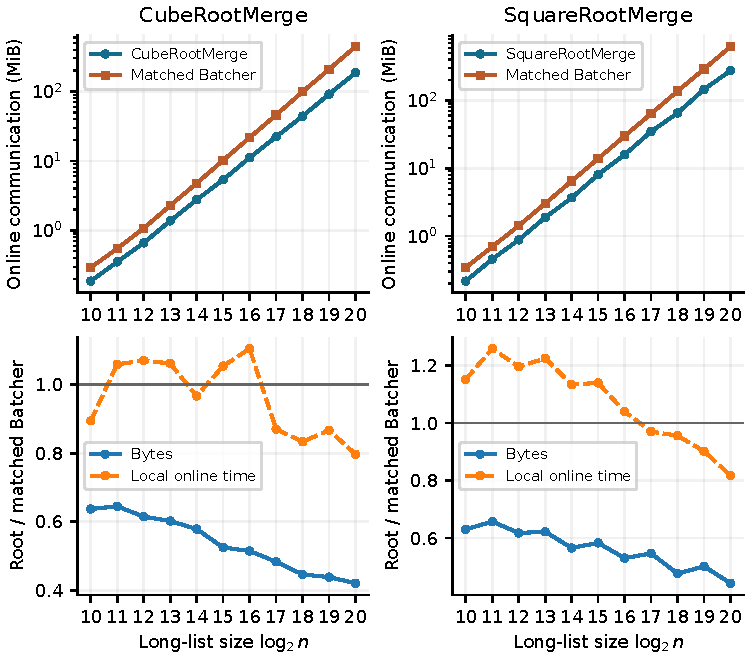
\includegraphics[width=\linewidth]{plots/root/root-merge-communication.pdf}
\caption{Online communication and ratios to matched unequal-length Batcher.
The ratio panels also show local online time. The horizontal line denotes
equality; connecting lines guide the eye.}
\label{fig:root-communication}
\end{figure}

\begin{table}[!htbp]
\centering\small
\setlength{\tabcolsep}{3pt}
\begin{tabular}{llrrrrr}
\hline
Shape & Protocol & Online & Offline & Local & Local & Depth \\
 & & MiB & MiB & online s & offline s & \\
\hline
Cube & Root & 186.3 & 862.0 & 0.461 & 44.33 & 109 \\
Cube & Batcher & 443.3 & 248.4 & 0.578 & 56.95 & 168 \\
\hline
Square & Root & 275.3 & 1022.0 & 0.724 & 60.36 & 210 \\
Square & Batcher & 622.4 & 348.7 & 0.886 & 80.05 & 168 \\
\hline
\end{tabular}

\caption{Asymmetric merges at long-list size $n=2^{20}$. Cube uses $m=102$;
Square uses $m=1024$. Times are medians of three local executions.
Communication includes both parties. Depth excludes preprocessing.}
\label{tab:root-large}
\end{table}

\begin{figure}[!htbp]
\centering
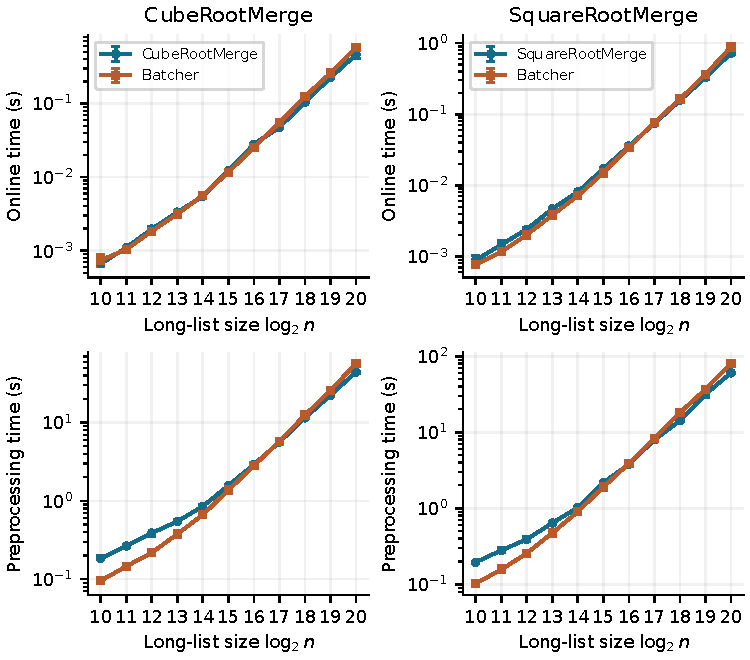
\includegraphics[width=\linewidth]{plots/root/root-merge-local.pdf}
\caption{Local online and preprocessing times for both asymmetric shapes.
Each marker is a three-run median with its observed range. Both parties
execute on one OS thread.}
\label{fig:root-local}
\end{figure}

\clearpage
\paragraph{Network sensitivity and preprocessing.}
We emulate LAN (1\,Gbit/s, 0.2\,ms RTT) and WAN (100\,Mbit/s, 40\,ms RTT)
links using isolated Linux network namespaces and a virtual Ethernet pair.
Each direction receives a \texttt{tc netem} rate limit and half the specified
RTT. Both endpoints run on this laptop. We take three matched executions
on both profiles at $n=2^{12}$ and $2^{16}$ and on WAN at $n=2^{20}$.
TCP phase time is the slower endpoint's time. Offline-plus-online time sums
these phase times per execution before taking the median.
An unloaded calibration measures mean RTTs of 0.270 and 40.597\,ms and
receiver TCP goodput of approximately 957 and 95.7\,Mbit/s for LAN and WAN,
respectively. The artifact retains the per-direction measurements and
interface offload settings.

At $n=2^{20}$, CubeRootMerge ($m=102$, $b=128$) sends 186.32\,MiB online versus 443.30\,MiB for matched Batcher, a 58.0\% reduction. Its local online median is 0.461\,s (range 0.415--0.466), versus 0.578\,s (0.573--0.608).
On the emulated WAN, the online medians are 13.199 and 25.139\,s, respectively (1.90$\times$ speedup). Including preprocessing, the medians are 90.91 and 87.11\,s.

At $n=2^{20}$, SquareRootMerge ($m=1024$, $b=512$) sends 275.25\,MiB online versus 622.44\,MiB for matched Batcher, a 55.8\% reduction. Its local online median is 0.724\,s (range 0.688--0.726), versus 0.886\,s (0.885--0.915).
On the emulated WAN, the online medians are 20.018 and 33.836\,s, respectively (1.69$\times$ speedup). Including preprocessing, the medians are 118.66 and 120.57\,s.



The online gains do not imply a uniform improvement in total time.
At $2^{20}$, CubeRootMerge's WAN total is higher than Batcher's, while the
observed total-time ranges for SquareRootMerge and Batcher overlap.
At $2^{12}$, SquareRootMerge is slower online on WAN despite communicating
fewer bytes: its greater depth dominates on this small, latency-sensitive case.
Figure~\ref{fig:root-network} retains these smaller-size comparisons.

\begin{figure}[!htbp]
\centering
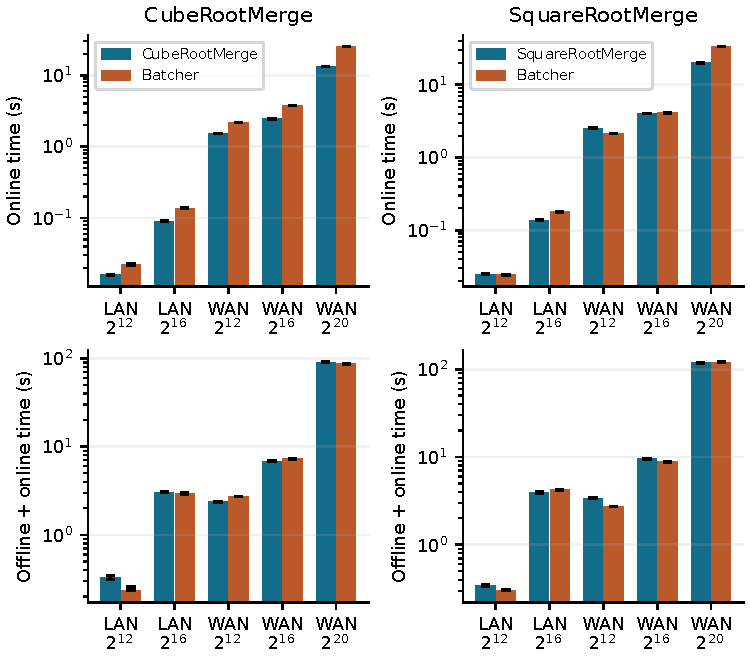
\includegraphics[width=\linewidth]{plots/root/root-merge-network.pdf}
\caption{Measured TCP online and offline-plus-online times for matched
asymmetric merges. Bars are three-run medians; error bars show observed
ranges. Rates are full-duplex caps per direction.}
\label{fig:root-network}
\end{figure}

Preprocessing generates GMW multiplication correlations and the two sets of
masked permutation correlations. Our online refinements do not remove the
permutation generator's OT/VOLE and PRF work. Accordingly, the artifact records
offline communication and time alongside every online measurement, as well as
peak memory and sampled swap. The implementation opportunities discussed in
Section~\ref{sec:packed-offline} also apply here; we make no quantitative claim
about unimplemented offline improvements. The raw records, selected parameters,
verification results, and plotting scripts are included in the artifact.
\clearpage

% END ASYMMETRIC ROOT-MERGE EVALUATION
